\pdfoptionpdfminorversion=7
\documentclass{beamer}

\mode<presentation>
{
  \usetheme{Madrid}       % or try default, Darmstadt, Warsaw, ...
  \usecolortheme{default} % or try albatross, beaver, crane, ...
  \usefonttheme{serif}    % or try default, structurebold, ...
  \setbeamertemplate{navigation symbols}{}
  \setbeamertemplate{caption}[numbered]
}

\usepackage{amsmath}

\usepackage[utf8x]{inputenc}
\usepackage{graphicx}
\usepackage{listings}
\usepackage{lmodern}

\title{Proyecto de titulo X}
\author{Yerko Zec}
\institute[]{FI - UNAB}
\date{2019/08/13}

\begin{document}

\begin{frame}[plain]
  \titlepage
\end{frame}

\addtocounter{framenumber}{-1}

\begin{frame}{Nuevos Ligandos}
\begin{itemize}
 \item Se ha logrado obtener nuevos ligandos.
 \item Los problemas que se han presentado son ...
 \item Se concluye que ...
\end{itemize}

\begin{figure}
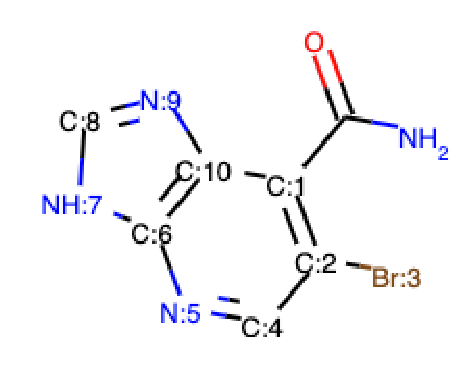
\includegraphics[width=0.3\linewidth]{newLigand}
\end{figure}
\end{frame}

\begin{frame}{Trabajo Futuro}
\begin{itemize}
 \item Tareas por hacer para abordar los problemas.
 \item Tareas futuras por hacer.
\end{itemize}
\end{frame}
\end{document}
